\usepackage{palatino}
%\usepackage[lite,subscriptcorrection,slantedGreek,nofontinfo]{mtpro2}
%\usepackage{eulervm}
%\usepackage{dsfont}
\usepackage{array}
%\usepackage{fontspec}
\usepackage{tabularx}
\usepackage{multirow}

\theoremstyle{definition}
\newtheorem{property}{Property}
\newtheorem{lemmarm}{Lemma}
\newtheorem{corollaryrm}{Corollary}
\newtheorem{question}{Question}

\newtheorem{observation}{Observation}
\usepackage{environ}
\usepackage{tabularx}
\usepackage{graphviz}
\usepackage{dashbox}
\usepackage{lscape}
%\usepackage{enumitem}
\usepackage{amssymb}
\usepackage{amsmath}

\usepackage{xspace}
\usepackage{graphicx}
\usepackage{url}
\usepackage{cite}
\usepackage{color}
\usepackage{pgfplots}

\usepackage{palatino}
%\usepackage[lite,subscriptcorrection,slantedGreek,nofontinfo]{mtpro2}
%\usepackage{eulervm}
\usepackage{dsfont}
\usepackage{array}
\usepackage{amssymb}
\usepackage{amsthm}
\usepackage{amsmath}
%\usepackage{fontspec}
\usepackage{tabularx}
\usepackage{multirow}
\usepackage{environ}
\usepackage{pgfplots}

\newcommand{\eqdef}{\stackrel{\text{def}}{=}}





% Math
\newcommand{\B}{\mathds{B}}
\newcommand{\bbbb}{\ensuremath{\mathrm{I\!B}}}
%\newcommand{\bbbf}{\ensuremath{\mathrm{I\!F}}}
\newcommand{\bfunc}{\ensuremath{\mathcal{B}}}
\newcommand{\T}{\ensuremath{\mathrm{T}}}





% Toffoli gate
\def\T{\mathrm{T}}

% @ Operator
\DeclareMathOperator{\at}{@}

% Bra-ket
\def\|#1>{\ensuremath{|#1\rangle}}

\def\|#1>{\left|#1\right\rangle}
\def\<#1|{\left\langle#1\right|}


\usepackage{tikz}

\usepackage{listings}


\usetikzlibrary{calc,trees,positioning,arrows,chains,shapes.geometric,%
    decorations.pathreplacing,decorations.pathmorphing,shapes,%
    matrix,shapes.symbols}
\usetikzlibrary{arrows,automata}
\usetikzlibrary{backgrounds,calc,decorations.pathreplacing,positioning}
\usepackage{verbatim}

\tikzset{%
  font=\scriptsize,>=latex,
  block2/.style={draw,rectangle,minimum height=7.6cm,minimum width=9cm,align=center, rounded corners,fill=white,opacity=.9,draw=none},
  block12/.style={draw,rectangle,dashed, text width=1.8cm, text centered,rounded corners, minimum height=1em , align=center} ,
  block/.style    = { rectangle, draw=blue, thick, fill=blue!20, text width=1.8cm, text centered,rounded corners, minimum height=1em },
  line/.style     = { draw, thick, ->, shorten >=2pt }  
}
\definecolor{RAblue}{RGB}{4,78,134}
\definecolor{green1}{rgb}{0.000000,0.392157,0.000000}
\tikzset{
>=stealth,
  punktchain/.style={
    rectangle, 
    rounded corners, 
    % fill=black!10,
    draw=black, very thick,
    text width=10em, 
    minimum height=3em, 
    text centered, 
    on chain},
  line/.style={draw, thick, <-},
  element/.style={
    tape,
    top color=white,
    bottom color=blue!50!black!60!,
    minimum width=8em,
    draw=blue!40!black!90, very thick,
    text width=10em, 
    minimum height=3.5em, 
    text centered, 
    on chain},
  every join/.style={->, thick,shorten >=1pt},
  decoration={brace},
  tuborg/.style={decorate},
  tubnode/.style={midway, right=2pt},
}
\tikzstyle{decision} = [diamond, draw, fill=blue!20, 
    text width=2em, text badly centered, node distance=3cm, inner sep=0pt]
\tikzstyle{block} = [rectangle, draw, fill=blue!20, 
    text width=6em, text centered, rounded corners, minimum height=1.5em]
\tikzstyle{line} = [draw, -latex']
\tikzstyle{cloud} = [draw, ellipse,fill=red!20, node distance=2cm,
    minimum height=2em]

%##########################################################################################################################################
\newcommand{\fancyarrow}[3]{%
  \expandafter\ifnum#2<180\def\outAngle{90}\else\def\outAngle{270}\fi
  \expandafter\ifnum#2<90\def\inAngle{180}\def\endDelta{1pt}\else\expandafter\ifnum#2>270\def\inAngle{180}\def\endDelta{1pt}\else\def\inAngle{0}\def\endDelta{-1pt}\fi\fi
  \draw[RAred!80!white,thick,<-] #1 coordinate (t) to[out=\outAngle,in=\inAngle] +(#2:#3) coordinate (s);
  \fill[RAred!80!white] (t) to[out=\outAngle,in=\inAngle] ([xshift=\endDelta,yshift=1.5pt] s) -- (s) -- ([xshift=\endDelta,yshift=-1.5pt] s) to[out=\inAngle,in=\outAngle] (t);
}


\tikzset{%
	font=\footnotesize,
	>=stealth,
	flow item/.style={draw,inner sep=2pt,text height=1.5ex,text depth=.25ex}
}

\newcommand{\tikzTripleStoreExtraction}{%
	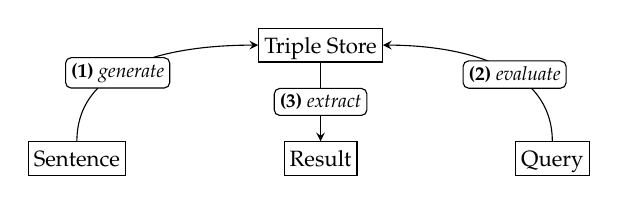
\begin{tikzpicture}
	\begin{scope}[every node/.style={flow item}]
	\begin{scope}[start chain,every node/.append style={on chain},node distance=2cm]
	\node (sentence) {Sentence};
	\node (result) {Result};
	\node (query) {Query};
	\end{scope}
	\node[above=of result] (store) {Triple Store};
	\end{scope}
	
	\begin{scope}[every node/.style={pos=.4,font=\scriptsize,inner sep=2pt,draw,rounded corners=2pt,fill=white}]
	\draw[->] (sentence.north) to[out=90,in=180] node {\textbf{(1)} \textit{generate}} (store.west);
	\draw[->] (query.north) to[out=90,in=0] node {\textbf{(2)} \textit{evaluate}} (store.east);
	\draw[->] (store.south) to node[midway] {\textbf{(3)} \textit{extract}} (result.north);
	\end{scope}
	\end{tikzpicture}
}

\newcommand{\tikzFlow}{%
	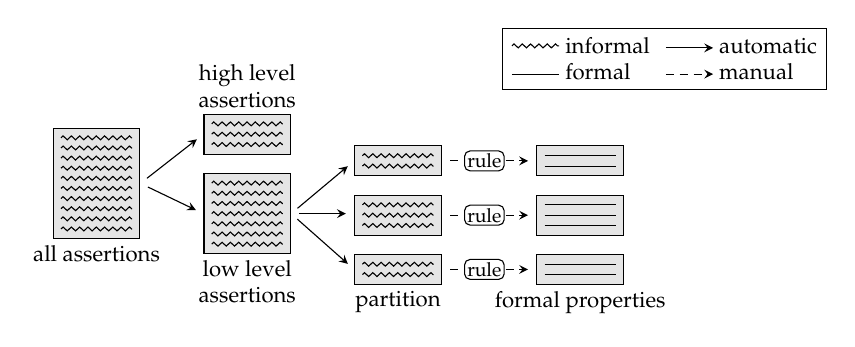
\begin{tikzpicture}
	\begin{scope}[every node/.style={draw,minimum width=1.1cm,fill=gray!20!white}]
	\node[minimum height=1.4cm] (all assertions) {};
	\node[minimum height=.51cm,anchor=north west] at ([xshift=.8cm,yshift=.18cm] all assertions.north east) (hl assertions) {};
	\node[minimum height=1.02cm,anchor=north west] at ([yshift=-.23cm] hl assertions.south west) (ll assertions) {};
	\node[minimum height=.38cm,anchor=north west] at ([xshift=.8cm,yshift=.35cm] ll assertions.north east) (g1 assertions) {};
	\node[minimum height=.51cm,anchor=north west] at ([yshift=-.23cm] g1 assertions.south west) (g2 assertions) {};
	\node[minimum height=.38cm,anchor=north west] at ([yshift=-.23cm] g2 assertions.south west) (g3 assertions) {};
	
	\node[minimum height=.38cm,anchor=north west] at ([xshift=1.2cm] g1 assertions.north east) (g1 properties) {};
	\node[minimum height=.51cm,anchor=north west] at ([yshift=-.23cm] g1 properties.south west) (g2 properties) {};
	\node[minimum height=.38cm,anchor=north west] at ([yshift=-.23cm] g2 properties.south west) (g3 properties) {};
	\end{scope}
	
	\begin{scope}[decoration={zigzag,amplitude=.7pt,segment length=3pt}]
	\foreach \n/\t/\ti in {all assertions/10/11,hl assertions/3/4,ll assertions/7/8,g1 assertions/2/3,g2 assertions/3/4,g3 assertions/2/3} {%
		\foreach \y in {1,...,\t} {%
			\draw[decorate] ([xshift=3pt]  $(\n.north west)!\y/\ti!(\n.south west)$)
			-- ([xshift=-3pt] $(\n.north east)!\y/\ti!(\n.south east)$);
		}
	}
	\end{scope}
	\foreach \n/\t/\ti in {g1 properties/2/3,g2 properties/3/4,g3 properties/2/3} {%
		\foreach \y in {1,...,\t} {%
			\draw ([xshift=3pt]  $(\n.north west)!\y/\ti!(\n.south west)$)
			-- ([xshift=-3pt] $(\n.north east)!\y/\ti!(\n.south east)$);
		}
	}
	
	\begin{scope}[every node/.style={inner sep=2pt,align=center}]
	\node[below] at (all assertions.south) {all assertions};
	\node[above] at (hl assertions.north) {high level \\ assertions};
	\node[below] at (ll assertions.south) {low level \\ assertions};
	\node[below] at (g3 assertions.south) {partition};
	\node[below] at (g3 properties.south) {formal properties};
	\end{scope}
	
	\begin{scope}[->,shorten <=3pt,shorten >=3pt,every node/.style={pos=.45,font=\scriptsize,fill=white,inner sep=1pt,draw,rounded corners=2pt,solid}]
	\draw (all assertions.east) -- (hl assertions.west);
	\draw (all assertions.east) -- (ll assertions.west);
	\draw (ll assertions.east) -- (g1 assertions.west);
	\draw (ll assertions.east) -- (ll assertions.east -| g2 assertions.west);
	\draw (ll assertions.east) -- (g3 assertions.west);
	\draw[densely dashed] (g1 assertions.east) -- node {rule} (g1 properties.west);
	\draw[densely dashed] (g2 assertions.east) -- node {rule} (g2 properties.west);
	\draw[densely dashed] (g3 assertions.east) -- node {rule} (g3 properties.west);
	\end{scope}
	
	\coordinate (c) at (current bounding box.center);
	\coordinate (d) at ($(c)+(.5\linewidth,0)$);
	\coordinate (e) at ([yshift=.4cm] d |- current bounding box.north east);
	\node[anchor=north east,align=left,draw] at (e) {%
		\raise.5ex\hbox{\tikz \draw[decoration={zigzag,amplitude=.7pt,segment length=3pt},decorate] (0,0) -- ++(right:.6cm);} \hbox to 1.2cm {informal}
		\raise.5ex\hbox{\tikz \draw[->] (0,0) -- ++(right:.6cm);} automatic \\
		\raise.5ex\hbox{\tikz \draw (0,0) -- ++(right:.6cm);} \hbox to 1.2cm {formal}
		\raise.5ex\hbox{\tikz \draw[densely dashed,->] (0,0) -- ++(right:.6cm);} manual
	};
	
	% \begin{pgfonlayer}{background}
	%   \draw[ultra thick,gray!50!white] (c) -- ++(left:.5\linewidth)
	%                                    (c) -- ++(right:.5\linewidth);
	% \end{pgfonlayer}
	\end{tikzpicture}
}

\newcommand\tikzActiveO{%
	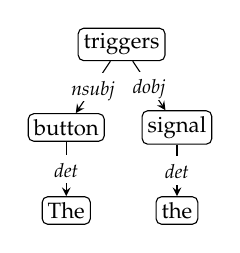
\begin{tikzpicture}[v/.style={draw,inner sep=2pt,rounded corners=2pt,%
		font=\footnotesize},%
	e/.style={inner sep=1pt,fill=white,text height=1.5ex,%
		text depth=.25ex,font=\scriptsize\itshape}]
	\node[v] (triggers-3) {triggers}
	[sibling distance=40pt,level distance=30pt]
	child[->] {node[v] {button}
		child[->] {node[v] {The} edge from parent node[e] {det}}
		edge from parent node[e] {nsubj}
	}
	child[->] {node[v] {signal}
		child[->] {node[v] {the} edge from parent node[e] {det}}
		edge from parent node[e] {dobj}
	};
	\end{tikzpicture}
}

\newcommand\tikzPassiveO{%
	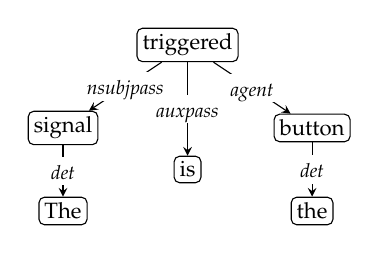
\begin{tikzpicture}[v/.style={draw,inner sep=2pt,rounded corners=2pt,%
		font=\footnotesize},%
	e/.style={inner sep=1pt,fill=white,text height=1.5ex,%
		text depth=.25ex,font=\scriptsize\itshape}]
	\node[v] (triggers-3) {triggered}
	[sibling distance=45pt,level distance=30pt]
	child[->] {node[v] {signal}
		child[->] {node[v] {The} edge from parent node[e] {det}}
		edge from parent node[e] {nsubjpass}
	}
	child[->,level distance=45pt] {node[v] {is} edge from parent node[e] {auxpass}}
	child[->] {node[v] {button}
		child[->] {node[v] {the} edge from parent node[e] {det}}
		edge from parent node[e] {agent}
	};
	\end{tikzpicture}
}

\newcommand\tikzTwoDependencyGraphs{%
	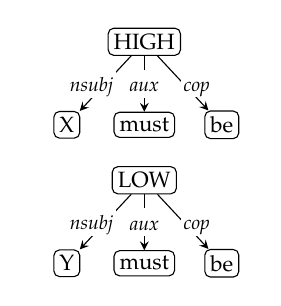
\begin{tikzpicture}[v/.style={draw,inner sep=2pt,rounded corners=2pt,%
		font=\footnotesize},%
	e/.style={inner sep=1pt,fill=white,text height=1.5ex,%
		text depth=.25ex,font=\scriptsize\itshape}]
	\node[v] (high) {HIGH}
	[sibling distance=28pt,level distance=30pt]
	child[->] {node[v] {X} edge from parent node[e,xshift=-5pt] {nsubj}}
	child[->] {node[v] {must} edge from parent node[e] {aux}}
	child[->] {node[v] {be} edge from parent node[e,xshift=5pt] {cop}};
	
	\node[v,below=1.4cm of high] {LOW}
	[sibling distance=28pt,level distance=30pt]
	child[->] {node[v] {Y} edge from parent node[e,xshift=-5pt] {nsubj}}
	child[->] {node[v] {must} edge from parent node[e] {aux}}
	child[->] {node[v] {be} edge from parent node[e,xshift=5pt] {cop}};
	
	% enlarge picture
	\begin{pgfonlayer}{background}
	\draw[white] ([xshift=-1.5cm] current bounding box.center) --
	([xshift=1.5cm] current bounding box.center);
	\end{pgfonlayer}
	\end{tikzpicture}
}

\newcommand\tikzRepresentativeGraph{%
	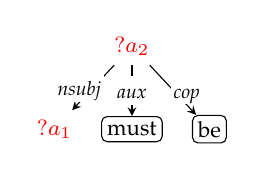
\begin{tikzpicture}[v/.style={draw,inner sep=2pt,rounded corners=2pt,%
		font=\footnotesize},%
	var/.style={font=\footnotesize\color{red}},%
	e/.style={inner sep=1pt,fill=white,text height=1.5ex,%
		text depth=.25ex,font=\scriptsize\itshape}]
	\node[var] {$?a_2$}
	[sibling distance=28pt,level distance=30pt]
	child[->] {node[var] {$?a_1$} edge from parent node[e,xshift=-5pt] {nsubj}}
	child[->] {node[v] {must} edge from parent node[e] {aux}}
	child[->] {node[v] {be} edge from parent node[e,xshift=5pt] {cop}};
	\end{tikzpicture}
}

\newcommand\tikzDependenciesList{%
	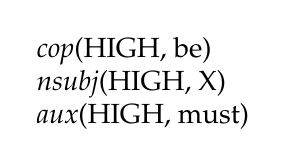
\begin{tikzpicture}
	\node[align=left,font=\baselineskip12pt] {%
		\textit{cop}(HIGH, be) \\
		\textit{nsubj}(HIGH, X) \\
		\textit{aux}(HIGH, must)
	};
	\end{tikzpicture}
}

\newcommand\tikzDependenciesGraph{%
	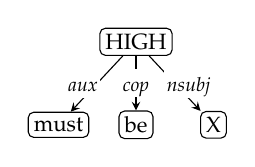
\begin{tikzpicture}[v/.style={draw,inner sep=2pt,rounded corners=2pt,%
		font=\footnotesize},%
	e/.style={inner sep=1pt,fill=white,text height=1.5ex,%
		text depth=.25ex,font=\scriptsize\itshape}]
	\node[v] {HIGH}
	[sibling distance=28pt,level distance=30pt]
	child[->] {node[v] {must} edge from parent node[e,xshift=-5pt] {aux}}
	child[->] {node[v] {be} edge from parent node[e] {cop}}
	child[->] {node[v] {X} edge from parent node[e,xshift=5pt] {nsubj}};
	\end{tikzpicture}
}

\newcommand\tikzCanonDeps{%
	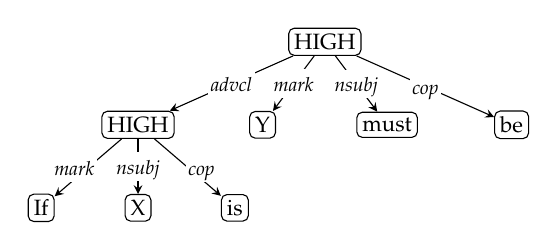
\begin{tikzpicture}[v/.style={draw,inner sep=2pt,rounded corners=2pt,%
		font=\footnotesize},%
	e/.style={inner sep=1pt,fill=white,text height=1.5ex,%
		text depth=.25ex,font=\scriptsize\itshape}]
	\node[v] {HIGH}
	[sibling distance=45pt,level distance=30pt]
	child[->] {node[v] {HIGH}
		[sibling distance=35pt,level distance=30pt]
		child[->] {node[v] {If} edge from parent node[e,xshift=-5pt] {mark}}
		child[->] {node[v] {X} edge from parent node[e] {nsubj}}
		child[->] {node[v] {is} edge from parent node[e,xshift=5pt] {cop}}
		edge from parent node[e] {advcl}}
	child[->] {node[v] {Y} edge from parent node[e] {mark}}
	child[->] {node[v] {must} edge from parent node[e] {nsubj}}
	child[->] {node[v] {be} edge from parent node[e] {cop}};
	\end{tikzpicture}
}

\newcommand\tikzAssertionTemplate{%
	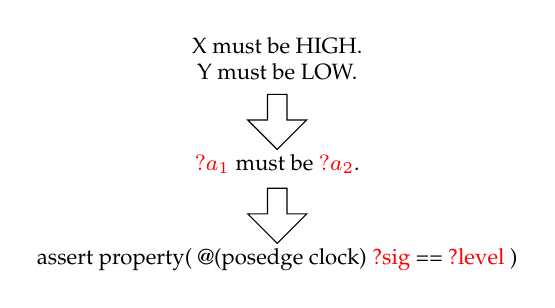
\begin{tikzpicture}
	\begin{scope}[start chain=going below,every node/.style={on chain},node distance=.7cm]
	\node[align=center] (a) {%
		X must be HIGH. \\
		Y must be LOW.
	};
	
	\node (b) {{\color{red}$?a_1$} must be {\color{red}$?a_2$}.};
	
	\node (c) {%
		assert property( @(posedge clock) {\color{red}?sig} == {\color{red}?level} )
	};
	\end{scope}
	
	\node[draw,single arrow,shape border rotate=270,minimum height=.7cm] at ($(a.south)!.5!(b.north)$) {};
	\node[draw,single arrow,shape border rotate=270,minimum height=.7cm] at ($(b.south)!.5!(c.north)$) {};
	\end{tikzpicture}
}

%##########################################################################################################################################
\newcommand{\slideOutline}{
\begin{enumerate}
\item Motivation\pause
\item \pause
\item \pause
\item \pause
\item 	
\end{enumerate}	
}
%##########################################################################################################################################
\newcommand{\slideMotivation}{%
\vspace{-0.58cm}
\begin{tikzpicture}[auto,>=latex]


 \node [name=circuit]{};
 
 \node [right of= circuit,node distance=0 cm] (ref){\tikzDesignFlow};
 \visible<5->{ \node [block2,right of= ref,node distance=0 cm] (O){};}
\node [right of= ref,node distance=3 cm] (O){};
 \visible<6->{ \node [below of= ref,node distance=0.1 cm] (O){
\includegraphics[width=.35\linewidth]{images/images5.jpg}};}
 \end{tikzpicture}

}
    
%##########################################################################################################################################
\newcommand{\slideMotivationVersion}{
 \begin{columns}
 \begin{column}{.33\textwidth}

\begin{center}
\visible<1->{\includegraphics[width=.7\linewidth]{images/images0.jpg}}
\end{center}
    \end{column}
    
  \begin{column}{.33\textwidth}
\begin{center}
  \vspace{-1.cm}
 \visible<2->{\includegraphics[width=.5\linewidth]{images/images1.jpg}}\\
   \vspace{1.cm}
  \visible<5->{ \includegraphics[width=.8\linewidth]{images/images5.jpg}}\\
   \vspace{1.cm}
 \visible<4->{ \includegraphics[width=.5\linewidth]{images/error_icon.jpg}}\\
\end{center}
\end{column}

  \begin{column}{.33\textwidth}
 
\begin{center}
\visible<3->{ \includegraphics[width=.6\linewidth]{images/images33.jpg}}
\end{center}
\end{column}
\end{columns}


}
 
 %##########################################################################################################################################
\newcommand{\slideMotivationOne}{
\vspace{-3}
\includegraphics[width=.3\linewidth]{images/images34.jpg}

}
 %##########################################################################################################################################
\newcommand{\slideSolution}{
 \begin{columns}
 \begin{column}{.33\textwidth}
 
\begin{center}
Writing Specification\\\vspace{0.3cm}
\includegraphics[width=.5\linewidth]{images/images1.jpg}\pause
\end{center}
    \end{column}
    
  \begin{column}{.33\textwidth}
\begin{center}
\vspace{0.5cm}
 \includegraphics[width=.3\linewidth]{images/images2.jpg}\pause\\

\end{center}
\end{column}

  \begin{column}{.33\textwidth}
\vspace{-0.3cm}
\begin{center}
Quality Validation\\
 \includegraphics[width=.6\linewidth]{images/images9.jpg}
\end{center}
\end{column}
\end{columns}

}

    
       
%##########################################################################################################################################
\newcommand{\slideConsequences}{
\begin{flushleft}
Better Writen specification will:  \pause
\end{flushleft}
\begin{itemize}
\item improve the comprehensibility of the designer\pause
\item enhance the quality of automatic extraction approaches
\end{itemize}}
    

 %##########################################################################################################################################
\newcommand{\slideApproach}{
	\vspace{-1cm}
\begin{enumerate}
%	\renewcommand{\labelenumi}{\textbf{\arabic{enumi}.}}
	\item Requirement quality based on: \pause
	
	\begin{itemize}
		\item Syntactic Quality \pause
		\item Semantic Quality\pause
	\end{itemize}
	\item	Assertions translation approach
\end{enumerate}}
%##########################################################################################################################################
\newcommand{\slideFirstApproachOne}{
  \vspace{-1cm}
 \begin{problem}[Sentence quality]
  Given an English sentence, the \emph{sentence quality} problem asks to
  determine a quality measure indicating whether the sentence is \emph{good},
  \emph{medium}, or \emph{bad} in terms of comprehension.
  \end{problem}

}   

%##########################################################################################################################################
\newcommand{\slideFirstApproachTwo}{ 
  \vspace{-1cm}
\begin{enumerate}
	%\renewcommand{\labelenumi}{\textbf{\arabic{enumi}.}}
\item Requirement quality based on: \pause

\begin{itemize}
\item Syntactic Quality \pause
\item Semantic Quality\pause
\end{itemize}
\item	Assertions translation approach
\end{enumerate}
}   
%##########################################################################################################################################
\newcommand{\slideSyntactic}{ 
  \vspace{-1cm}
\begin{flushleft}
It is considered as directly ambivalent to the number of structural ambiguities.  %Therefore, the smaller the number of structural ambiguities is, the better is the syntactic quality 
 \pause
\end{flushleft}
\begin{itemize}
\item Calculation based on phrase structure trees \pause
\item \emph{Isomorphic subtrees} \pause
\item \emph{Sentence length penalty}
\end{itemize}
}   %##########################################################################################################################################
\newcommand{\slideSemanticOne}{ 

  \begin{itemize}
\item It is determined by its amount of semantic ambiguities\\\pause
\item WordNet is used to determine that\pause
\item A word is ambiguous if it has more than one \textit{synsets} in the WordNet dictionary\pause
\item A \textit{synsets} is a set of cognitive synonyms
  \end{itemize}
  } 
%##########################################################################################################################################
\newcommand{\slideSemanticTwo}{ 
  \begin{flushleft}
let :\pause
  \end{flushleft}
\begin{itemize}
\item $n$ be the number of nonambiguous words\pause
\item $m$ be the number of ambiguous words\pause
\item $a = n/(n+m)$ be the distinct portion of the sentence\pause
\item $b = m/(n+m)$ be the ambiguous portion of the sentence\pause
%\item  $a+b=1$, If $a=1$ then the  sentence is free of ambiguities\pause
\item  $k_i$ be the number of different synsets of the $i$-th ambiguous word\pause
\end{itemize}

\begin{flushleft}
Then the basic semantic quality is given by:\pause
\end{flushleft}
\begin{equation}
  \label{eq:semantic-quality}
  q_{\rm sem}=a + b\cdot \frac{m}{\sum_{i=1}^mk_i}.
\end{equation}

}  
%##########################################################################################################################################



\newcommand{\slideDataBaseOne}{%
 \begin{flushleft}
The requirements database is taken from: \pause
\end{flushleft}
\begin{itemize}
\item NASA hardware requirement specifications\pause
\item Intel hardware requirement specifications.\pause
\item Random hardware requirement specifications
\end{itemize}
}
%##########################################################################################################################################
\newcommand{\slideExperimental}{ 
  \vspace{-1cm}
   \begin{table}[h]
  \centering
  \small
   \def\tabcolsep{5pt}
  \begin{tabularx}{\linewidth}{X|rrrrr|r} \hline
    \textbf{Quality} & \textbf{Algo.} & \textbf{Subj.} & \textbf{Matches} & \textbf{Misses} & \textbf{Misses} & \textbf{Matching} \\
    \textbf{predicate} & & & & \textbf{dist. 1} & \textbf{dist. 2} & \textbf{percentage}\\\hline
    good&32&26&20&8&4&62.5 \% \\
    medium&53&41&29&24&$\times$&54.7 \%\\
    bad&37&55&31&4&2&83.8 \%\\\hline
    total&122&122&80&36&6&65.6 \% \\\hline
  \end{tabularx}
  \end{table}
}  


%##########################################################################################################################################
\newcommand{\slideSecondApproachOne}{
  \vspace{-1cm}
\begin{problem}[Guideline checking]
  Given a set of rules from guidelines how to write requirements and a natural
  language requirement~$R$, the \emph{guideline checking} problem asks whether
  $R$ adheres to the rules.
\end{problem}
}   
  %##########################################################################################################################################
\newcommand{\slideSecondApproachTwo}{
  \vspace{-1cm}
\begin{flushleft}
Requirement quality Evaluation based on:  \pause
\end{flushleft}
\begin{itemize}
\item Rule based approach \pause
\item Stanford CoreNP
\item Scala programming language
\end{itemize}
}  
%##########################################################################################################################################
\newcommand{\slideExtractedRules}{%
 \begin{flushleft}
The rules are extracted from: \pause
\end{flushleft}
\begin{itemize}

\item NASA guidelines\pause
\item IBM guidelines.\pause
\item "Writing Better Requirement", I. Alexander and R. Stevens
\end{itemize}
  
}
  
  
  
  
%##########################################################################################################################################
\newcommand{\slideRules}{%
\begin{enumerate}
  %\renewcommand{\labelenumi}{\textbf{R\arabic{enumi}.}}
\item Define one requirement at a time.\pause
\item Avoid conjunctions (and, or, with, also) that make multiple requirements.\pause
\item Use simple direct sentences.\pause
\item Each requirement must contain a subject and a predicate.\pause
\item Avoid let-out clauses (unless, except, if necessary, but, when, unless, although).\pause
\item Avoid expressing suggestions or possibilities (might, may, could, ought, should, could, perhaps, probably).
\end{enumerate}
  }
%##########################################################################################################################################
\newcommand{\slideRulesTwo}{%
\begin{enumerate}
\setcounter{enumi}{6}
 % \renewcommand{\labelenumi}{\textbf{R\arabic{enumi}.}}
\item Avoid weak phrases and undefined terms (adequate, as a minimum, as applicable, easy, as appropriate, be able to, be capable, but not limited to, capability of, capability to, effective, if practical, normal, provide for, timely, tbd, user-friendly, versatile, robust, approximately, minimal impact, etc., and so on, flexible, to the maximum extent, as much as possible, minimal impact, in one whack, different, various, many, some of, diverse)\pause
\item Do not speculate (usually, generally, often, normally, typically).\pause
\item Avoid wishful thinking (100\% reliable, safe, handle all failures, fully upgradeable, run on all platforms).\pause
\item Define verifiable criteria.
\end{enumerate}
  }

%##########################################################################################################################################
\newcommand{\slideImplementationOne}{%
   \vspace{-2.78cm}
\begin{flushleft}
    \textbf{R1.}  Define one requirement at a time.\\\pause
\end{flushleft}
  \vspace{0.2cm}
      \textbf{the system is reset at start-up.\\}\pause
       \vspace{0.2cm} 
\includegraphics[width=.6\linewidth]{images/image_parse_tree.png}

}
%##########################################################################################################################################
\newcommand{\slideImplementationTwo}{%
   \vspace{-0.5cm}
\begin{flushleft}
    \textbf{R1.}  Define one requirement at a time.\\
\end{flushleft}
  \vspace{0.2cm}
      \textbf{the system is reset at start-up.\\}
\includegraphics[width=.45\linewidth]{images/parse_tree.png}\pause
\begin{flushleft}
Cheeking the phrase structure tree whether it has two sentences related directly to the root.
\end{flushleft}
}
%##########################################################################################################################################


\newcommand{\slideImplementationThree}{%
  \vspace{-1cm}
  \begin{flushleft}
  \textbf{R3.} Use simple direct sentences.\\\pause
  
  
\end{flushleft}
 \begin{columns}
 \begin{column}{.4\textwidth}
\begin{center}
 Active voice\\
  \tikzActive \pause
\end{center}
    \end{column}
  \begin{column}{.6\textwidth}
\begin{center}

  Passive voice\\
  \tikzPassive
\end{center}
\end{column}
\end{columns}

}

%##########################################################################################################################################
\newcommand{\slideDataBaseTwo}{%

The requirements database is the same as the one used in the first approach.
}


%##########################################################################################################################################
\newcommand{\slideResults}{%
 
  \begin{table}[h]
 \def\tabcolsep{3pt}
 \small
\centering
\begin{tabularx}{\linewidth}{X|rr|rr|rrrrr|r}
	\hline
	\multicolumn{1}{l|}{\textbf{Rules}} & \multicolumn{2}{c|}{\textbf{M. Class.}} & \multicolumn{2}{c|}{\textbf{A. Class.}} &  \multicolumn{6}{c}{\textbf{Classifier Evaluation }} \\
	& \multicolumn{1}{r}{T} & \multicolumn{1}{r|}{F} & \multicolumn{1}{r}{T} & \multicolumn{1}{r|}{F}& \multicolumn{1}{c}{SA}& \multicolumn{1}{c}{TP} & \multicolumn{1}{c}{TN} & \multicolumn{1}{c}{FP} & \multicolumn{1}{c|}{FN}& \multicolumn{1}{c}{Acc.}\\ \hline
	\textbf{R1} & 88 & 15 & 61 & 42 & 70 & 58 & 12 & 30 & 3 & 67.96\% \\ 
	\textbf{R2} & 84 & 19 & 89 & 14 & 80 & 75 & 5 & 9 & 14 & 77.67\% \\ 
	\textbf{R3} & 90 & 13 & 89 & 14 & 86 & 81 & 5 & 9 & 8 & 83.50\% \\ 
	\textbf{R4} & 102 & 1 & 92 & 11 & 93 & 92 & 1 & 10 & 0 & 90.29\% \\ 
	\textbf{R5} & 94 & 9 & 95 & 8 & 102 & 94 & 8 & 0 & 1 & 99.03\% \\ 
	\textbf{R6} & 92 & 11 & 85 & 18 & 92 & 83 & 9 & 9 & 2 & 89.32\% \\ 
	\textbf{R7} & 102 & 1 & 103 & 0 & 102 & 102 & 0 & 0 & 1 & 99.03\% \\ 
	\textbf{R8} & 103 & 0 & 103 & 0 & 103 & 103 & 0 & 0 & 0 & 100.00\% \\ 
	\textbf{R9} & 9 & 17 & 18 & 8 & 13 & 7 & 6 & 2 & 11 & 50.00\% \\  \hline
	\textbf{Total} & 826 & 127 & 772 & 181 & 811 & 728 & 83 & 98 & 44 & 82.48\% \\ 
	\hline
\end{tabularx}
\end{table}
}


\newcommand{\slideResultsTwo}{%

\begin{table}[t]
	\def\tabcolsep{3pt}
	\centering
	
	\label{tab4}
	\begin{tabularx}{\linewidth}{X|rr|rr|rrrrr|r}
		\hline
		\multicolumn{1}{l|}{\textbf{Rules}} & \multicolumn{2}{c|}{\textbf{M. Class.}} & \multicolumn{2}{c|}{\textbf{A. Class.}} &  \multicolumn{6}{c}{\textbf{Classifier Evaluation }} \\
		& \multicolumn{1}{r}{T} & \multicolumn{1}{r|}{F} & \multicolumn{1}{r}{T} & \multicolumn{1}{r|}{F}& \multicolumn{1}{c}{SA}& \multicolumn{1}{c}{TP} & \multicolumn{1}{c}{TN} & \multicolumn{1}{c}{FP} & \multicolumn{1}{c|}{FN}& \multicolumn{1}{c}{Acc.}\\ \hline
		\textbf{R1} & 52 & 32 & 54 & 30 & 76 & 49 & 27 & 3 & 5 & 90.48\% \\ 
		\textbf{R2} & 68 & 16 & 35 & 49 & 45 & 32 & 13 & 36 & 3 & 53.57\% \\ 
		\textbf{R3} & 31 & 53 & 19 & 65 & 62 & 14 & 48 & 17 & 5 & 73.81\% \\ 
		\textbf{R4} & 76 & 8 & 76 & 8 & 80 & 74 & 6 & 2 & 2 & 95.24\% \\ 
		\textbf{R5} & 77 & 7 & 75 & 9 & 80 & 74 & 6 & 3 & 1 & 95.24\% \\ 
		\textbf{R6} & 65 & 19 & 61 & 23 & 78 & 60 & 18 & 5 & 1 & 92.86\% \\ 
		\textbf{R7} & 82 & 2 & 80 & 4 & 82 & 80 & 2 & 2 & 0 & 97.62\% \\ 
		\textbf{R8} & 84 & 0 & 84 & 0 & 84 & 84 & 0 & 0 & 0 & 100.00\% \\ 
		\textbf{R9} & 26 & 8 & 27 & 7 & 19 & 19 & 0 & 7 & 8 & 55.88\% \\ \hline
		\textbf{Total} & 589 & 201 & 541 & 249 & 680 & 510 & 170 & 79 & 31 & 84.28\% \\  \hline
	\end{tabularx}
\end{table}
}

\newcommand{\slideResultsThree}{%
	\begin{itemize}
		\item SA= Number of the Same annotated requirement
		\item TP+FP= Number of manual True  annotated requirements
		\item TN+FN= Number of manual false  annotated requirements
		\item Acc=$\frac{\mathrm{TP}+\mathrm{TN}}
		{\mathrm{TP}+\mathrm{TN}+\mathrm{FP}+\mathrm{FN}}$
	\end{itemize}
}	
	
%##########################################################################################################################################
\newcommand{\slideTranslation}{%
	\vspace{-1cm}
	\begin{flushleft}
			Proposed flow
	\end{flushleft} \pause
			\vspace{1cm}
\tikzFlow
	
}   
\newcommand{\slideAlogorithmZero}{%
	\begin{enumerate}
	%	\renewcommand{\labelenumi}{\textbf{\arabic{enumi}.}}
		\item Abstraction Level Classification\pause
		\item Partitioning based on Sentence Similarity\pause
		\item Assertion Generation
	\end{enumerate}	
}  

\newcommand{\slideAlogorithmOne}{%
	\vspace{-1cm}
	Using A SPARQL query to partition the assertion into \pause
	\begin{itemize}
	 \item high abstraction level subsets\pause
	 \item low abstraction level subsets
\end{itemize}
}  


\newcommand{\slideAlogorithmTwo}{%
	\vspace{-1cm}
	\begin{columns}
		\begin{column}{.5\textwidth}
		 \begin{center}
		 	\tikzTwoDependencyGraphs
		 \end{center} \pause
		\end{column}
		\begin{column}{.5\textwidth}
			 \begin{center}
			 	\tikzRepresentativeGraph
			 \end{center}
		\end{column}
	\end{columns}	
}  
\newcommand{\slideAlogorithmThree}{%
	\vspace{-1cm}
	\begin{enumerate}
	%	\renewcommand{\labelenumi}{\textbf{\arabic{enumi}.}}
		\item an assertion template is generated for each cluster\pause
		\item the assertion template is populated for each natural language assertion in the cluster.	
	\end{enumerate}
}  
\newcommand{\slideExperResOne}{%
	\begin{flushleft}
		The algorithm is applied to the assertions is taken from: \pause
	\end{flushleft}
	\begin{itemize}
		\item AMBA 3 AXI Protocol Checker user guide containing 145 assertions\pause	
		\item Random hardware assertion list\pause	
	\end{itemize}
	\begin{flushleft}
		Requirement quality Evaluation based on:  \pause
	\end{flushleft}
	\begin{itemize}
		\item Stanford CoreNP \pause
		\item JENA API for the triple store based information extraction
	\end{itemize}}
	
\newcommand{\slideExperResTwo}{%
\begin{enumerate}
	%\renewcommand{\labelenumi}{\textbf{\arabic{enumi}.}}
	\item Abstraction Level Classification\pause 
\begin{itemize}
	\item From 145 assertions 100 have been classified as low level assertions\pause
\end{itemize}

\item Partitioning based on Sentence Similarity\pause
\begin{itemize}
	\item  11 clusters are found\pause
\end{itemize}
\item Partitioning based on Sentence Similarity\pause
\begin{itemize}
 		\item 11 SystemVerilog assertion templates were generated \pause
 		\item Each is applied to all elements of the corresponding cluster
\end{itemize}	
\end{enumerate}
}
%##########################################################################################################################################
\newcommand{\slideConclusion}{%
  \vspace{-1cm}
\begin{flushleft}
Two Requirement evaluation approaches\pause
\end{flushleft}
  \begin{itemize}
\item Static Sentence Analysis\pause
\item Guidelines Validation\pause
\end{itemize}
\begin{flushleft}
	Assertions translation approach
\end{flushleft}
}   

%##########################################################################################################################################
\newcommand{\slideFutureWork}{%
  \vspace{-2cm}
\begin{itemize}
\item Fixing violating rules requirement\pause
\item Semi automatic technique 
\end{itemize}
}   

%##########################################################################################################################################

\newcommand\tikztreeParsing{%
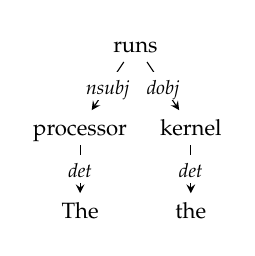
\begin{tikzpicture}[v/.style={draw=none,inner sep=2pt,rounded corners=2pt,%
                    font=\footnotesize,text height=1.5ex,text depth=.25ex},%
                    e/.style={inner sep=1pt,fill=white,text height=1.5ex,%
                    text depth=.25ex,font=\scriptsize\itshape}]
  \node[v] (triggers-3) {runs}
    [sibling distance=40pt,level distance=30pt]
    child[->] {node[v] {processor}
      child[->] {node[v] {The} edge from parent node[e] {det}}
      edge from parent node[e] {nsubj}
    }
    child[->] {node[v] {kernel}
      child[->] {node[v] {the} edge from parent node[e] {det}}
      edge from parent node[e] {dobj}
    };
\end{tikzpicture}
}
%##########################################################################################################################################


\newcommand\tikzActive{%
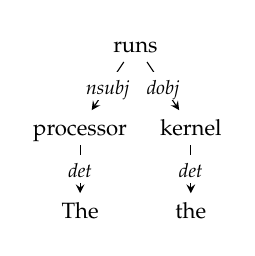
\begin{tikzpicture}[v/.style={draw=none,inner sep=2pt,rounded corners=2pt,%
                    font=\footnotesize,text height=1.5ex,text depth=.25ex},%
                    e/.style={inner sep=1pt,fill=white,text height=1.5ex,%
                    text depth=.25ex,font=\scriptsize\itshape}]
  \node[v] (triggers-3) {runs}
    [sibling distance=40pt,level distance=30pt]
    child[->] {node[v] {processor}
      child[->] {node[v] {The} edge from parent node[e] {det}}
      edge from parent node[e] {nsubj}
    }
    child[->] {node[v] {kernel}
      child[->] {node[v] {the} edge from parent node[e] {det}}
      edge from parent node[e] {dobj}
    };
\end{tikzpicture}
}
%##########################################################################################################################################

\newcommand\tikzPassive{%
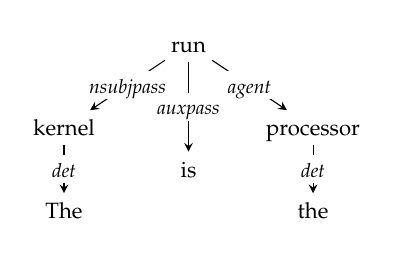
\begin{tikzpicture}[v/.style={draw=none,inner sep=2pt,rounded corners=2pt,%
                    font=\footnotesize,text height=1.5ex,text depth=.25ex},%
                    e/.style={inner sep=1pt,fill=white,text height=1.5ex,%
                    text depth=.25ex,font=\scriptsize\itshape}]
  \node[v] (triggers-3) {run}
    [sibling distance=45pt,level distance=30pt]
    child[->] {node[v] {kernel}
      child[->] {node[v] {The} edge from parent node[e] {det}}
      edge from parent node[e] {nsubjpass}
    }
    child[->,level distance=45pt] {node[v] {is} edge from parent node[e] {auxpass}}
    child[->] {node[v] {processor}
      child[->] {node[v] {the} edge from parent node[e] {det}}
      edge from parent node[e] {agent}
    };
\end{tikzpicture}
}
%##########################################################################################################################################

\newcommand\tikzDesignFlow{
\begin{tikzpicture}[->,>=stealth',shorten >=1pt,auto,node distance=4.3cm,
  thick,main node/.style={draw=none,font=\sffamily\Large\bfseries}]

\visible<2->{  \node[main node] (1) {\includegraphics[width=.15\linewidth]{images/images1.jpg}};}
\visible<1->{  \node[main node] (2) [below left of=1] {\includegraphics[width=.2\linewidth]{images/images0.jpg}};}
\visible<4->{  \node[main node] (3) [below right of=2] {\includegraphics[width=.1\linewidth]{images/error_icon.jpg}};}
\visible<3->{   \node[main node] (4) [below right of=1] {\includegraphics[width=.16\linewidth]{images/images33.jpg}};}

\visible<2->{  \path[every node/.style={font=\sffamily\small,text centered}, color  = RAblue, ]
  (2) edge [bend left] node[left, text width=2cm] {Wrting Spec.} (1);}\visible<3->{
   \path[every node/.style={font=\sffamily\small,text centered}, color  = RAblue, ]
   (1)  edge [bend left] node[text width=2.0cm] {Designing} (4)   ;}
\visible<4->{
   \path[every node/.style={font=\sffamily\small,text centered}, color  = RAblue, ](4) edge [bend left] node[right, text width=1.5cm] {Error Detecting} (3);}
 
\end{tikzpicture}}

% Local Variables:
% mode: latex
% TeX-master: "talk"
% End:


%%% Local Variables:
%%% mode: latex
%%% TeX-master: "talk"
%%% End:
